%%%%%%%%%%%%%%%%%%%%%%%%%%%%%%%%%%%%%%%%%%%%%%%%%%%%%%%%%%%%%%%%%%%%%%%%%%
%
% 	Template for seminar reports
%
%%%%%%%%%%%%%%%%%%%%%%%%%%%%%%%%%%%%%%%%%%%%%%%%%%%%%%%%%%%%%%%%%%%%%%%%%%

%%%%%%%%%%%%%%%%%%%%%%%%%%%%%%%%%%%%%%%%%%%%%%%%%%%%%%%%%%%%%%%%%%%%%%%%%%
% 	Include layout and macros
%%%%%%%%%%%%%%%%%%%%%%%%%%%%%%%%%%%%%%%%%%%%%%%%%%%%%%%%%%%%%%%%%%%%%%%%%%


%% This LaTeX template is based on the following example file included in the ieeetran
%% package:
%% bare_conf.tex 
%% V1.2
%% 2002/11/18
%% by Michael Shell
%% mshell@ece.gatech.edu
%% (requires IEEEtran.cls version 1.6b or later) with an IEEE conference paper.


% Note that the a4paper option is mainly intended so that authors in
% countries using A4 can easily print to A4 and see how their papers will
% look in print. Authors are encouraged to use U.S. letter paper when 
% submitting to IEEE. Use the testflow package mentioned above to verify
% correct handling of both paper sizes by the author's LaTeX system.
%
% Also note that the "draftcls" or "draftclsnofoot", not "draft", option
% should be used if it is desired that the figures are to be displayed in
% draft mode.
%
% This paper can be formatted using the peerreviewca
% (instead of conference) mode.
\documentclass[conference, a4paper]{IEEEtran-modified}
% If the IEEEtran.cls has not been installed into the LaTeX system files, 
% manually specify the path to it:
% \documentclass[conference]{../sty/IEEEtran} 

\IEEEoverridecommandlockouts

% some very useful LaTeX packages include:

\usepackage{cite}       % Written by Donald Arseneau
                        % V1.6 and later of IEEEtran pre-defines the format
                        % of the cite.sty package \cite{} output to follow
                        % that of IEEE. Loading the cite package will
                        % result in citation numbers being automatically
                        % sorted and properly "ranged". i.e.,
                        % [1], [9], [2], [7], [5], [6]
                        % (without using cite.sty)
                        % will become:
                        % [1], [2], [5]--[7], [9] (using cite.sty)
                        % cite.sty's \cite will automatically add leading
                        % space, if needed. Use cite.sty's noadjust option
                        % (cite.sty V3.8 and later) if you want to turn this
                        % off. cite.sty is already installed on most LaTeX
                        % systems. The latest version can be obtained at:
                        % http://www.ctan.org/tex-archive/macros/latex/contrib/supported/cite/

%\usepackage{graphicx}  % Written by David Carlisle and Sebastian Rahtz
                        % Required if you want graphics, photos, etc.
                        % graphicx.sty is already installed on most LaTeX
                        % systems. The latest version and documentation can
                        % be obtained at:
                        % http://www.ctan.org/tex-archive/macros/latex/required/graphics/
                        % Another good source of documentation is "Using
                        % Imported Graphics in LaTeX2e" by Keith Reckdahl
                        % which can be found as esplatex.ps and epslatex.pdf
                        % at: http://www.ctan.org/tex-archive/info/
% NOTE: for dual use with latex and pdflatex, instead load graphicx like:
\ifx\pdfoutput\undefined
	\usepackage{graphicx}
\else
	\usepackage[pdftex]{graphicx}
\fi

% However, be warned that pdflatex will require graphics to be in PDF
% (not EPS) format and will preclude the use of PostScript based LaTeX
% packages such as psfrag.sty and pstricks.sty. IEEE conferences typically
% allow PDF graphics (and hence pdfLaTeX). However, IEEE journals do not
% (yet) allow image formats other than EPS or TIFF. Therefore, authors of
% journal papers should use traditional LaTeX with EPS graphics.
%
% The path(s) to the graphics files can also be declared: e.g.,
% \graphicspath{{../eps/}{../ps/}}
% if the graphics files are not located in the same directory as the
% .tex file. This can be done in each branch of the conditional above
% (after graphicx is loaded) to handle the EPS and PDF cases separately.
% In this way, full path information will not have to be specified in
% each \includegraphics command.
%
% Note that, when switching from latex to pdflatex and vice-versa, the new
% compiler will have to be run twice to clear some warnings.
\graphicspath{{figures/}}


%\usepackage{psfrag}    % Written by Craig Barratt, Michael C. Grant,
                        % and David Carlisle
                        % This package allows you to substitute LaTeX
                        % commands for text in imported EPS graphic files.
                        % In this way, LaTeX symbols can be placed into
                        % graphics that have been generated by other
                        % applications. You must use latex->dvips->ps2pdf
                        % workflow (not direct pdf output from pdflatex) if
                        % you wish to use this capability because it works
                        % via some PostScript tricks. Alternatively, the
                        % graphics could be processed as separate files via
                        % psfrag and dvips, then converted to PDF for
                        % inclusion in the main file which uses pdflatex.
                        % Docs are in "The PSfrag System" by Michael C. Grant
                        % and David Carlisle. There is also some information 
                        % about using psfrag in "Using Imported Graphics in
                        % LaTeX2e" by Keith Reckdahl which documents the
                        % graphicx package (see above). The psfrag package
                        % and documentation can be obtained at:
                        % http://www.ctan.org/tex-archive/macros/latex/contrib/supported/psfrag/

%\usepackage{subfigure} % Written by Steven Douglas Cochran
                        % This package makes it easy to put subfigures
                        % in your figures. i.e., "figure 1a and 1b"
                        % Docs are in "Using Imported Graphics in LaTeX2e"
                        % by Keith Reckdahl which also documents the graphicx
                        % package (see above). subfigure.sty is already
                        % installed on most LaTeX systems. The latest version
                        % and documentation can be obtained at:
                        % http://www.ctan.org/tex-archive/macros/latex/contrib/supported/subfigure/

%\usepackage{url}       % Written by Donald Arseneau
                        % Provides better support for handling and breaking
                        % URLs. url.sty is already installed on most LaTeX
                        % systems. The latest version can be obtained at:
                        % http://www.ctan.org/tex-archive/macros/latex/contrib/other/misc/
                        % Read the url.sty source comments for usage information.

%\usepackage{stfloats}  % Written by Sigitas Tolusis
                        % Gives LaTeX2e the ability to do double column
                        % floats at the bottom of the page as well as the top.
                        % (e.g., "\begin{figure*}[!b]" is not normally
                        % possible in LaTeX2e). This is an invasive package
                        % which rewrites many portions of the LaTeX2e output
                        % routines. It may not work with other packages that
                        % modify the LaTeX2e output routine and/or with other
                        % versions of LaTeX. The latest version and
                        % documentation can be obtained at:
                        % http://www.ctan.org/tex-archive/macros/latex/contrib/supported/sttools/
                        % Documentation is contained in the stfloats.sty
                        % comments as well as in the presfull.pdf file.
                        % Do not use the stfloats baselinefloat ability as
                        % IEEE does not allow \baselineskip to stretch.
                        % Authors submitting work to the IEEE should note
                        % that IEEE rarely uses double column equations and
                        % that authors should try to avoid such use.
                        % Do not be tempted to use the cuted.sty or
                        % midfloat.sty package (by the same author) as IEEE
                        % does not format its papers in such ways.

\usepackage{amsmath}    % From the American Mathematical Society
                        % A popular package that provides many helpful commands
                        % for dealing with mathematics. Note that the AMSmath
                        % package sets \interdisplaylinepenalty to 10000 thus
                        % preventing page breaks from occurring within multiline
                        % equations. Use:
\interdisplaylinepenalty=2500
                        % after loading amsmath to restore such page breaks
                        % as IEEEtran.cls normally does. amsmath.sty is already
                        % installed on most LaTeX systems. The latest version
                        % and documentation can be obtained at:
                        % http://www.ctan.org/tex-archive/macros/latex/required/amslatex/math/



% Other popular packages for formatting tables and equations include:

%\usepackage{array}
% Frank Mittelbach's and David Carlisle's array.sty which improves the
% LaTeX2e array and tabular environments to provide better appearances and
% additional user controls. array.sty is already installed on most systems.
% The latest version and documentation can be obtained at:
% http://www.ctan.org/tex-archive/macros/latex/required/tools/

% Mark Wooding's extremely powerful MDW tools, especially mdwmath.sty and
% mdwtab.sty which are used to format equations and tables, respectively.
% The MDWtools set is already installed on most LaTeX systems. The lastest
% version and documentation is available at:
% http://www.ctan.org/tex-archive/macros/latex/contrib/supported/mdwtools/


% V1.6 of IEEEtran contains the IEEEeqnarray family of commands that can
% be used to generate multiline equations as well as matrices, tables, etc.


% Also of notable interest:

% Scott Pakin's eqparbox package for creating (automatically sized) equal
% width boxes. Available:
% http://www.ctan.org/tex-archive/macros/latex/contrib/supported/eqparbox/



% Notes on hyperref:
% IEEEtran.cls attempts to be compliant with the hyperref package, written
% by Heiko Oberdiek and Sebastian Rahtz, which provides hyperlinks within
% a document as well as an index for PDF files (produced via pdflatex).
% However, it is a tad difficult to properly interface LaTeX classes and
% packages with this (necessarily) complex and invasive package. It is
% recommended that hyperref not be used for work that is to be submitted
% to the IEEE. Users who wish to use hyperref *must* ensure that their
% hyperref version is 6.72u or later *and* IEEEtran.cls is version 1.6b 
% or later. The latest version of hyperref can be obtained at:
%
% http://www.ctan.org/tex-archive/macros/latex/contrib/supported/hyperref/
%
% Also, be aware that cite.sty (as of version 3.9, 11/2001) and hyperref.sty
% (as of version 6.72t, 2002/07/25) do not work optimally together.
% To mediate the differences between these two packages, IEEEtran.cls, as
% of v1.6b, predefines a command that fools hyperref into thinking that
% the natbib package is being used - causing it not to modify the existing
% citation commands, and allowing cite.sty to operate as normal. However,
% as a result, citation numbers will not be hyperlinked. Another side effect
% of this approach is that the natbib.sty package will not properly load
% under IEEEtran.cls. However, current versions of natbib are not capable
% of compressing and sorting citation numbers in IEEE's style - so this
% should not be an issue. If, for some strange reason, the user wants to
% load natbib.sty under IEEEtran.cls, the following code must be placed
% before natbib.sty can be loaded:
%
% \makeatletter
% \let\NAT@parse\undefined
% \makeatother
%
% Hyperref should be loaded differently depending on whether pdflatex
% or traditional latex is being used:
%
%\ifx\pdfoutput\undefined
%\usepackage[hypertex]{hyperref}
%\else
%\usepackage[pdftex,hypertexnames=false]{hyperref}
%\fi
%
% Pdflatex produces superior hyperref results and is the recommended
% compiler for such use.



% *** Do not adjust lengths that control margins, column widths, etc. ***
% *** Do not use packages that alter fonts (such as pslatex).         ***
% There should be no need to do such things with IEEEtran.cls V1.6 and later.


\usepackage{ngerman}

\usepackage{amsmath}
\usepackage{algorithm}
\usepackage[noend]{algpseudocode}
\usepackage{graphicx}
\usepackage{url}
\usepackage[T1]{fontenc}

%%%%%%%%%%%%%%%%%%%%%%%%%%%%%%%%%%%%%%%%%%%%%%%%%%%%%%%%%%%%%%%%%%%%%%%%%%
% 	Page numbering (not on first page)
%%%%%%%%%%%%%%%%%%%%%%%%%%%%%%%%%%%%%%%%%%%%%%%%%%%%%%%%%%%%%%%%%%%%%%%%%%
\pagestyle{empty}

%%%%%%%%%%%%%%%%%%%%%%%%%%%%%%%%%%%%%%%%%%%%%%%%%%%%%%%%%%%%%%%%%%%%%%%%%%
% 	Correct bad hyphenation here
%%%%%%%%%%%%%%%%%%%%%%%%%%%%%%%%%%%%%%%%%%%%%%%%%%%%%%%%%%%%%%%%%%%%%%%%%%

\hyphenation{}

%%%%%%%%%%%%%%%%%%%%%%%%%%%%%%%%%%%%%%%%%%%%%%%%%%%%%%%%%%%%%%%%%%%%%%%%%%
% 	Begin of the document
%%%%%%%%%%%%%%%%%%%%%%%%%%%%%%%%%%%%%%%%%%%%%%%%%%%%%%%%%%%%%%%%%%%%%%%%%%

\begin{document}

%%%%%%%%%%%%%%%%%%%%%%%%%%%%%%%%%%%%%%%%%%%%%%%%%%%%%%%%%%%%%%%%%%%%%%%%%%
% 	Paper title
%%%%%%%%%%%%%%%%%%%%%%%%%%%%%%%%%%%%%%%%%%%%%%%%%%%%%%%%%%%%%%%%%%%%%%%%%%

\title{Evaluation of Topic Models for Supervised Word-Sense Disambiguation}

%%%%%%%%%%%%%%%%%%%%%%%%%%%%%%%%%%%%%%%%%%%%%%%%%%%%%%%%%%%%%%%%%%%%%%%%%%
% 	Author names and affiliations 
%		-	multiple columns for up to three different affilitations are separated 
%			by \and
%		- for over three affiliations, refer to ieeetran howto
%%%%%%%%%%%%%%%%%%%%%%%%%%%%%%%%%%%%%%%%%%%%%%%%%%%%%%%%%%%%%%%%%%%%%%%%%%

\author{
\authorblockN{Robert Br"unig}
\authorblockA{Fakult"at f"ur Informatik\\Technische Universit"at M"unchen\\
robert.bruenig@in.tum.de} 
\and
\authorblockN{Jakob Buchgraber}
\authorblockA{Fakult"at f"ur Informatik\\Technische Universit"at M"unchen\\
jakob.buchgraber@tum.de}
\and
\authorblockN{Philipp Dowling}
\authorblockA{Fakult"at f"ur Informatik\\Technische Universit"at M"unchen\\
dowling@in.tum.de}
}

%%%%%%%%%%%%%%%%%%%%%%%%%%%%%%%%%%%%%%%%%%%%%%%%%%%%%%%%%%%%%%%%%%%%%%%%%%
% 	Special paper note (appears between title and authors) 
%%%%%%%%%%%%%%%%%%%%%%%%%%%%%%%%%%%%%%%%%%%%%%%%%%%%%%%%%%%%%%%%%%%%%%%%%%

\specialpapernotice{Computerlinguistische Anwendungen}

%%%%%%%%%%%%%%%%%%%%%%%%%%%%%%%%%%%%%%%%%%%%%%%%%%%%%%%%%%%%%%%%%%%%%%%%%%
% 	Make title area 
%%%%%%%%%%%%%%%%%%%%%%%%%%%%%%%%%%%%%%%%%%%%%%%%%%%%%%%%%%%%%%%%%%%%%%%%%%

\maketitle

%%%%%%%%%%%%%%%%%%%%%%%%%%%%%%%%%%%%%%%%%%%%%%%%%%%%%%%%%%%%%%%%%%%%%%%%%%
% 	For page number on first page
%%%%%%%%%%%%%%%%%%%%%%%%%%%%%%%%%%%%%%%%%%%%%%%%%%%%%%%%%%%%%%%%%%%%%%%%%%

\thispagestyle{plain}

%%%%%%%%%%%%%%%%%%%%%%%%%%%%%%%%%%%%%%%%%%%%%%%%%%%%%%%%%%%%%%%%%%%%%%%%%%
% 	Abstract 
%%%%%%%%%%%%%%%%%%%%%%%%%%%%%%%%%%%%%%%%%%%%%%%%%%%%%%%%%%%%%%%%%%%%%%%%%%


\begin{abstract}
We present an evaluation of the performance that different topic models achieve when applied to the problem of supervised word-sense Disambiguation (WSD). Our algorithm was tested on the SensEval-3 English lexical sample task, using Latent Semantic Analysis (LSA) and Latent Dirichlet Allocation (LDA) at different dimensionalities, as well as the Hirearchical Dirichlet Process (HDP). All models were trained on the entire Wikipedia corpus, and applied in a variant on the Lesk algorithm. Our approach is based on selecting the word sense that most often occurs in the top \emph{k} most similar training instances. \\\\
Our results are on par with those of many of the entries to the SensEval-3 evaluation exercise. We found LSA at 350 topics (\emph{k = 12}) to perform best (\emph{recall 0.64}), with LSA generally outperforming LDA, and both outperforming HDP, which could not be properly evaluated partially due to time contraints.\\
\end{abstract}


%%%%%%%%%%%%%%%%%%%%%%%%%%%%%%%%%%%%%%%%%%%%%%%%%%%%%%%%%%%%%%%%%%%%%%%%%%
% 	Keywords 
%%%%%%%%%%%%%%%%%%%%%%%%%%%%%%%%%%%%%%%%%%%%%%%%%%%%%%%%%%%%%%%%%%%%%%%%%%

\begin{keywords}
topic model,
LSA,
LDA,
HDP,
word-sense disambiguation

\end{keywords}


%%%%%%%%%%%%%%%%%%%%%%%%%%%%%%%%%%%%%%%%%%%%%%%%%%%%%%%%%%%%%%%%%%%%%%%%%%
% 	Sections, Subsections,...
%%%%%%%%%%%%%%%%%%%%%%%%%%%%%%%%%%%%%%%%%%%%%%%%%%%%%%%%%%%%%%%%%%%%%%%%%%

\section{Introduction}
In this paper, we present an evaluation of the performance that different topic models achieve when applied to the problem of supervised word-sense Disambiguation (WSD) in a variation on the Lesk algorithm. 

\subsection{Supervised Word-Sense Disambiguation}
In virtually all languages, some words can have different meanings, or senses. WSD is the problem of determining  which sense of a word is being employed in a given context. In supervised WSD, both the words to be disambiguated and their possible senses are known beforehand, and labelled sample data is provided for each word sense. Consider the following example: The noun $atmosphere$ can, among other senses, refer to the air that surrounds the earth, as demonstrated by this sentence:\\
\begin{quotation}
\textit{Rising levels of greenhouse gas emissions are damaging the atmosphere.\\}
\end{quotation}
The term can also refer to the general mood surrounding an event. 
\begin{quotation}
\textit{Most attendees were in agreement that the party had a very pleasant atmosphere to it.\\}
\end{quotation}
Given sufficient data, supervised WSD systems should automatically determine the sense of a certain word in a new context. This is commonly done by training a classifier with feature vectors generated from the labelled data. State of the art systems for WSD currently achieve accuracies of over 90\% for certain tasks\cite{stateofart_scores}, however there are a number of different problem settings and top scores vary significantly based on the details of the task. For the SenseEval-3 English lexical sample task, which we also worked on, the top accuracies were around 72\%\cite{senseval3paper}.


\subsection{Topic Models}
Topic models are statistical models that aim to represent textual data as vectors in a topic-based vector space. Topic models have been applied to many different information retrieval and text clustering problems, but also in domains related to bioinformatics and other fields \cite{topicmodel_applications}. In essence, topic models learn patterns (topics) from unstructured data, in order to perform dimensionality reduction by converting term vectors into topic vectors. \\\\
A topic in this context is essentially a probability distribution over all words in the dictionary, with words that are relevant to the topic carrying positive weights, and the other words being assigned a weight very close to zero. Each dimension of the output vector then represents a weight of how well the document fits the particular topic. To train a topic model the respective set of model parameters is estimated from a large corpus through methods such as maximum likelihood or bayesian inference (in the form of maximum a posteriori (MAP) estimation). Most topic models are unsupervised algorithms.\\\\
As a result of this dimensional reduction, which respects the inferred semantic relations between words, topic models enable us to better compute document similarities. Even documents that share no words directly but regard a similar are likely to have similar vectors in topic space, even though their cosine similarity would be zero when considered as bag-of-words or TF-IDF vectors. In our experiments, we dealt with three specific topic models: Latent Semantic Analysis (LSA)\cite{LSA_paper}, Latent Dirichlet Allocation (LDA)\cite{LDA_paper}, and Hierarchical Dirichlet Process (HDP)\cite{HDP_paper}.


\subsection{Applications of Topic Models in WSD}
WSD algorithms usually involve either training classifiers, or computing similarities between contexts and glossaries (or other contexts). In both cases, topic models have strong potential applications. When training a classifier, the topic vectors themselves can be seen as features, and for computing simiarities topic models can provide much higher accuracy than more primitive methods like word overlap. Topic models have been applied to WSD in a number of different ways\cite{topic_models_in_wsd}. In fact, the LDA with \textsc{WordNet} (LDAWN) model was developed specifically for the problem of (unsupervised) WSD. \\
Our approach to supervised WSD employs topic models to improve the comparison of contexts between training and evaluation data. Contexts are converted into topic space, and on evaluation the context similarities are used to establish the most likely sense for the instance.

\section{Topic Models}
\subsection{Latent Semantic Analysis}

Latent Semantic Analysis (LSA) is a method that allows to identify topcis in unstructured text. It uses the bag of words model and the notion that words with similar meaning will occur in similar pieces of text. \\
When using LSA, one would typically construct a matrix $C$  with each row representing a unique word and each column representing a document or paragraph. The entry $C_{i,j}$ would then contain the number of occurrences of the (unique) word $i$ in the document $j$. In our particular implementation we chose to use the TF-IDF frequency instead of plain word counts, in an attempt to boost the relevance of rare words. The matrix $C$ will invariably be very sparse as each document only contains a tiny fraction of the total number of words. Furthermore, with large numbers of documents as input the matrix will also be of very high rank and simply be too massive to process or even fit in memory. LSA thus uses a mathematical technique called Singular Value Decomposition (SVD) to reduce the rank of the matrix to $k$, with $k$ usually being in the low hundreds. In short, the SVD of a matrix $C$ leads to three matrices so that $C = U{\Sigma}V^T$ is true, with $U$ and $V$ being orthogonal matrices and $\Sigma$ being a diagonal matrix. The entries $\Sigma_{i,i}$ are called the singular values with $U_{i}$ and $V_{i}$ being the left and right singular vectors respectively. The dimensionality reduction to rank $k$ then works by selecting the $k$ biggest singular values and the corresponding singular vectors $C_{k} = U_{k}{\Sigma_{k}}V_{k}$. This leads to a mathematical approximation of rank $k$ that has minimal error.\\\\

The resulting low dimensionality matrix $C_{k}$ is now referred to as \emph{semantic space} and finding similar words/topics boils down to computing the \emph{cosine distance} between two word vectors. A cosine value close to one means that the values are very similar (e.g. synonyms) while a value close to zero hints at words with different meaning.

\thispagestyle{plain}
\subsection{Latent Dirichlet Allocation}

Latent Dirichlet Allocation is a more sophisticated way of modelling and learning to discover topics in text. In contrast to LSA, LDA is a generative model that represents each document as a mixture of a small number of topics where each word in a document exists because it was generated by one of the document's topics. More specifically, LDA assumes that each document is generated in the following fashion:\\

\begin{enumerate}
    \item Determine the number of words $N$ in the document according to some probability distribution (e.g. Poisson).
    \item Select a mixture of $k$ topics for the document according to a Dirichlet distribution. Due to the lack of other evidence all $k$ parameters $\alpha_{i}$ of the distribution are set to the same $\alpha$.
    \item For each topic choose another parameter $\beta$ for the Dirichlet prior of the word distribution.
    \item Finally, generate each word by first picking a topic according to the multinomial distribution (as given by the chosen Dirichlet distribution) and second by using the topic's multinomial distribution to generate the word itself.\\
\end{enumerate}

Assuming this generative model, LDA then tries to backtrack from the documents to find the $k$ topics that have generated the document. More specifically, it tries to find the before mentioned multinomial distributions using Bayesian inference techniques such as Gibbs sampling and expectation propagation. 


\subsection{Hierarchical Dirichlet Process}

The Hierarchical Dirichlet Process is a non-parametric approach to topic models that utilizes similar underlying models to LDA. In fact, HDP can be considered a natural generalization of LDA with an unbound number of topics. The most important distinction of HDP to LDA (or LSA) is that the number of topics is not specified beforehand, but is instead learned from the data. This is achieved through utilizing nested Dirichlet processes - one for each document, with all processes sharing a common base distribution $H$, which is also drawn from a Dirichlet process\cite{HDP_paper}. \\\\
While HDP is referred to as a non-parametric method, there are in fact a few parameters that must be manually specified. These are related to the different Dirichlet processes and distributions utilized by the model. We will briefly discuss our settings of these parameters in section IV.
\thispagestyle{plain}
\section{Method}

% how the wsd proposed in this paper works:
% 	1. language model from wikipedia corpus
% 		-LDA & LSA
% 		-different dimensionalities
% 	2. labeled reference data
% 		-convert documents of reference data to topic vector space
% 		-save vector with sense id (=label)
% 	3. sense disambiguation
% 		-convert tested document to topic vector space
% 		-retrieve top k senseid using cosine measure from saved vector->senseid mapping
% 		-sense id of tested document is most frequent sense id in the top k retrieved


We created LSA, LDA and HDP topic models on the english wikipedia corpus (see \ref{creation}). To investigate the influence of topic count on the results, we  computed multiple instance of LDA and LSA models with different amounts of topics. Note that we do not include this step in our algorithm description - it is simply assumed that a trained topic model is already available.\\

Our algorithm consists of a training phase and an evaluation phase, however the training phase does not actually train a classifier. Instead, the contexts of all training instances are converted to the vector space of the topic model and is supsequently saved associated with the resepctive sense id.\\
The evaluation of a test instance is then done as follows. The test instance is also converted to the vector space of the topic model. Then, the top $k$ training contexts for the word in question are retrieved using the cosine similarity of the contexts. Finally, the sense id that occurs most frequently in the top $k$ results is chosen as the result for the test instance. Note that setting $k$ very high will simply result in always choosing the most frequent sense, which is in fact the baseline to which we measure the system's performance.\\

%initialize TM
%sense_vectors = Map()

%for each word in dictionary:
%	sense_vectors[word] = List()

%for each instance in train set:
%	vector = TM.convert(instance.vector)	
%	sense_vectors[instance.word].append(vector)
%

%for each instance in evaluation set:
%	candidates = sense_vectors[instance.word]
%	sort candidates by cosine similarity to TM.convert(instance)
% 	candidates = keep top k candidates
%	best_sense = most_frequent(candidates, k)
%	save this result
%
%
\begin{algorithm}[!t]
\caption{Word-Sense Disambiguation}\label{wsdalgorithm}
\begin{algorithmic}[1]
\State $\textit{initialize} \text{ TM} $
\State $\textit{sense\_vectors} := \textit{Map} {()}$
\Procedure{Train}{}
\ForAll {$instance \in train set$}
 \State$	vector := TM.convert(instance.bow)$
 \State$	sense\_vectors[instance.word].append(vector)$
\EndFor
%\State \Return $D_{comp}\cup D_{inc}$
\EndProcedure
\Procedure{Evaluate}{}
\State $\textit{results} := \textit{Map} {()}$
\ForAll {$instance \in evaluation set$}
 \State$	vector := TM.convert(instance.bow)$
 \State$	candidates := sense\_vectors[instance.word]$
 \State	sort candidates by cosine similarity to vector
 \State	cut off candidates at index k
 \State$	best\_sense := most\_frequent(candidates)$
 \State$	results[instance.id] := best\_sense$
 \State \Return $results$
\EndFor
%\State \Return $D_{comp}\cup D_{inc}$
\EndProcedure
\end{algorithmic}
\end{algorithm}

\subsection{Training of Topic Models}
\label{creation}
% details on data and how we created topic models
% 	1. wikipedia dumps
% 		-wikipedia does frequent dumps
% 		-we are using the latest dump of the articles in english wikipedia (as of june 2014) as xml
% 		-about 10GiB of compressed data, ~3.6 million documents
% 	2. topic model creationg
% 		-using gensim python library (decription of library)
% 		-gensim usage: lsa/lda interface, paramter description
% 		(-description of calculation time and machine hardware)
% 	3. additional models
% 		-hdp as test, implementation not mature therefore just used as test case
% 		-other models provided by gensim (random projections, log entropy) not used

For the training of a topic model large amounts of text are required. For providing that data we looked at the english Wikipedia. Wikipedia does frequent backups of its' articles and provides them for public use. We used the latest dump (as of june 2014) containing about 10GiB of compressed xml data or 3.6 million documents \cite{wikidumps}. The topic model was then trained using that data in an unsupervised manner.\\\\
The implementation of LSA, LDA and HDP topic models that we used was provided in the python library gensim. Gensim is a free, open-source library for topic modelling. For using the wikipedia dump with gensim, it first had to be preprocessed using TF-IDF. Gensim was then used to create LSA, LDA and HDP models with several dimensionalities from that corpus. We did not stem our training data, as this would have been very computationally expensive. In evaluation, the context data was therefore also not stemmed.\\\\
There are other topic models that are also supported by gensim that were not used for different reasons. Random projections (RP) \cite{RandomProjections, gensimRP} and log entropy (LE) \cite{LogEntropy, gensimLE} models were not used due to time contraints, but also because we did not expect them to outperform our other models. LE does not perform dimensionality reduction, and RP does not usually outperform LSA. 






\section{Experiments}
\subsection{Experimental Setup}
We used the SensEval-3 English lexical sample data as our training and evaluation set, so that we would be able to compare the performance of our approach to existing systems. The baseline performance for this task is to always choose the most frequent sense for each word.\\\\
We ran a large number of experiments at different parameters in order to find the optimal model and configuration. LSA was evaluated at 150, 200, 250, 300, 350 and 400 topics, each with a single pass over the corpus, two power iterations and no decay.\\\\
LDA was only evaluated at 200, 300 and 400 topics, since it is more computationally expensive to create those models. Here we used a symmetric prior of $\alpha = \frac{1}{n}$ for the per-document topic distribution, with the same value for $\beta$, the per-topic word distribution.\\\\
HDP was evaluated using the default parameters of Gensim: $\kappa = 1, \tau = 64, \alpha =1, \gamma =1, \eta =0.01$. Unfortunately, we were not able to properly use the HDP model, as the topics it generated did not appear make sense, and were all nearly identical. Due to time constraints we were not able to fix these issues and retrain the model. The results are nevertheless included in this paper.\\
\subsection{Results}
Figure 1 visualizes the results we obtained for different dimensionalities of LSA, LDA and the failed HDP attempt, together with the baseline performance. \\\\
%TODO: figure here.
As you can see, LSA appears to outperform LDA, and achieves its highest result of 0.641 at 350 topics with $k=10$. Other systems in SensEval-3 ranged from approximately 60\% to 73\% recall\cite{senseval-3}, so while our system is not on par with the state of the art in its current form, it performs reasonably well and has potential to be improved. 
\subsection{Outlook}
The algorithm presented here was fairly primitive, and serves mainly as a benchmark to compare the performance of different topic models for WSD. To optimize the systems performance, additionaly features may be considered and used to train a classifier of some sort. The entry $IRST-Kernels$ by the Team ITC-IRST at SensEval-3 was one of the highest performing systems, and used LSA in conjunction with paradiogmatic and syntagmatic information and other features in an SVM classifier\cite{IRSTkernels}. It is conceivable to achieve significantly higher performance by following similar methods, especially by considering local features in conjunction with LSA (which completely ignores local features).\\\\
There are also many more topic models that can be tried, as well as parameters in the training that can be tweaked. Going beyond topic models, any dimensionality reduction algorithm could be applied to this approach. For example, an interesting approach to consider might be marginalized Stacked Denoising Autoencoders (mSDA), which actually come from the field of deep learning but have in some benchmarks outperformed LDA in both accuracy and computational complexity.
% how did we score the diffent models
% 	1. scoring script provided, runs on test set, gives f-score/recall
% 	2. plotting tools / how were the graphics generated
% 	3. plot data: dimensionality against f-score
% 	4. interpretation of plots: what does that mean, how well did it perform


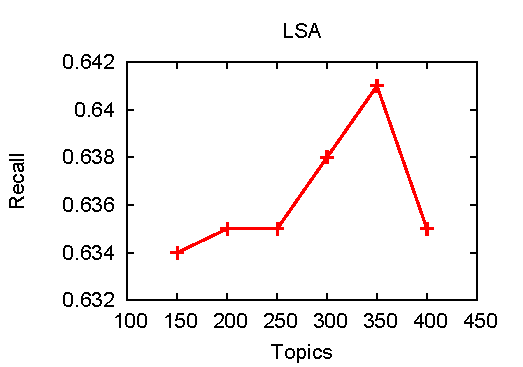
\includegraphics{plot/lsa_lines.pdf}

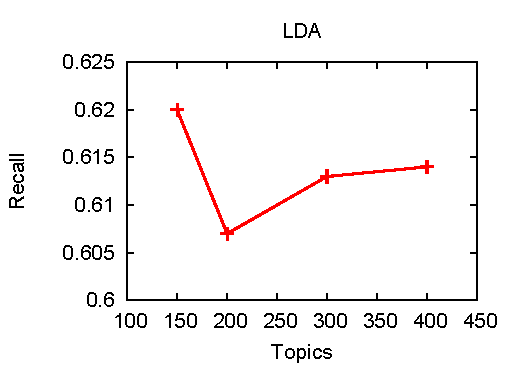
\includegraphics{plot/lda_lines.pdf}



\section{Conclusion}

We're awesome.
\thispagestyle{plain}
%%%%%%%%%%%%%%%%%%%%%%%%%%%%%%%%%%%%%%%%%%%%%%%%%%%%%%%%%%%%%%%%%%%%%%%%%%
% 	Acknowledgements
%%%%%%%%%%%%%%%%%%%%%%%%%%%%%%%%%%%%%%%%%%%%%%%%%%%%%%%%%%%%%%%%%%%%%%%%%%

%\section*{Acknowledgment}
%\addcontentsline{toc}{section}{Acknowledgment}

%%%%%%%%%%%%%%%%%%%%%%%%%%%%%%%%%%%%%%%%%%%%%%%%%%%%%%%%%%%%%%%%%%%%%%%%%%
% 	References
%%%%%%%%%%%%%%%%%%%%%%%%%%%%%%%%%%%%%%%%%%%%%%%%%%%%%%%%%%%%%%%%%%%%%%%%%%

% trigger a \newpage just before the given reference
% number - used to balance the columns on the last page
% adjust value as needed - may need to be readjusted if
% the document is modified later
%\IEEEtriggeratref{8}
% The "triggered" command can be changed if desired:
%\IEEEtriggercmd{\enlargethispage{-5in}}

% references section
% NOTE: BibTeX documentation can be easily obtained at:
% http://www.ctan.org/tex-archive/biblio/bibtex/contrib/doc/

% can use a bibliography generated by BibTeX as a .bbl file
% standard IEEE bibliography style from:
% http://www.ctan.org/tex-archive/macros/latex/contrib/supported/IEEEtran/bibtex
\bibliographystyle{IEEEtran}
% argument is your BibTeX string definitions and bibliography database(s)
\bibliography{IEEEabrv,references}
%
% <OR> manually copy in the resultant .bbl file
% set second argument of \begin to the number of references
% (used to reserve space for the reference number labels box)
%\begin{thebibliography}{1}
%
%\bibitem{ref:kopka}
%H.~Kopka and P.~W. Daly, \emph{A Guide to {\LaTeX}}, 3rd~ed.\hskip 1em plus
%  0.5em minus 0.4em\relax Harlow, England: Addison-Wesley, 1999.
%
%\end{thebibliography}

%%%%%%%%%%%%%%%%%%%%%%%%%%%%%%%%%%%%%%%%%%%%%%%%%%%%%%%%%%%%%%%%%%%%%%%%%%
% 	End of the document
%%%%%%%%%%%%%%%%%%%%%%%%%%%%%%%%%%%%%%%%%%%%%%%%%%%%%%%%%%%%%%%%%%%%%%%%%%

\end{document}


